\documentclass{llncs}

\usepackage{amsmath}
\usepackage{amssymb}
\usepackage{graphicx}
\usepackage{enumerate}
\usepackage{url}

\newcommand{\tup}[1]{\langle #1 \rangle}
\newcommand{\Omit}[1]{}
\newcommand{\vvec}[1]{\mathbf{#1}}
\newcommand{\join}{\bowtie}
\newcommand{\R}{\mathcal{R}}
\newcommand{\Q}{\mathcal{Q}}
\newcommand{\mcdsat}{\textsc{McdSat}}
\newcommand{\minicon}{{MiniCon}}

\newcommand{\qrule}{:\!\!-}
\newcommand{\orule}{\sqsubseteq}
\renewcommand{\L}{\mathcal{L}}
\newcommand{\M}{\mathcal{M}}

% Ontology concepts
\newcommand{\trip}{\textit{trip}}
\newcommand{\planetrip}{\textit{plane-trip}}
\newcommand{\traintrip}{\textit{train-trip}}
\newcommand{\AAflight}{\textit{AA-flight}}
\newcommand{\UAflight}{\textit{UA-flight}}
\newcommand{\ATtrain}{\textit{AT-train}}
\newcommand{\UPtrain}{\textit{UP-train}}
\newcommand{\flight}{\textit{flight}}
\newcommand{\train}{\textit{train}}
\newcommand{\UScity}{\textit{uscity}}

% Constants
\renewcommand{\AA}{\text{AA}}
\newcommand{\UA}{\text{UA}}
\newcommand{\AT}{\text{AT}}
\newcommand{\UP}{\text{UP}}
\newcommand{\PA}{\text{Paris}}
\newcommand{\NY}{\text{NY}}
\newcommand{\LA}{\text{LA}}
\newcommand{\AL}{\text{AL}}

% Services
\newcommand{\nationaltlight}{\textit{national-flight}}
\newcommand{\onewayflight}{\textit{one-way-flight}}
\newcommand{\nationaltrain}{\textit{national-train}}
\newcommand{\onewayTrain}{\textit{one-way-train}}
\newcommand{\onestop}{\textit{one-stop}}
\newcommand{\toPA}{\textit{to-pa}}
\newcommand{\onestopPA}{\textit{onestop-to-pa}}
\newcommand{\fromNY}{\textit{from-ny}}
\newcommand{\fromLA}{\textit{from-la}}

\begin{document}

\allowdisplaybreaks
\title{An Expressive and Efficient Solution to the Service Selection Problem}
\author{Daniel Izquierdo \and Mar\'{\i}a-Esther Vidal \and Blai Bonet}
\institute{Departamento de Computaci\'on \\
           Universidad Sim\'on Bol\'{\i}var \\
           Caracas 89000, Venezuela \\
           \url{{idaniel,mvidal,bonet}@ldc.usb.ve}}
\maketitle

\begin{abstract}
Given the large number of Semantic Web Services that can be created from
online sources by using existing annotation tools, expressive formalisms and
efficient and scalable approaches to solve the service selection problem are
required in order to make this services widely available to the users.
In this paper, we propose such a framework that is grounded on logic and
the Local-As-View approach for describing instances of the service selection problem.
In our approach, Web services are semantically described using LAV mappings
in terms of generic concepts from an ontology, while the user requests correspond
to conjunctive queries on the generic concepts, that must be combined to solve
a task, plus a set of preferences that are used to rank the possible solutions.
The LAV formulation allows us to cast the service selection problem as a
query rewriting problem that must consider the relationships among the concepts
in the ontology and the ranks induced by the preferences of the user.
Then, building on related work, we devise an encoding of the resulting
query rewriting problem as a logical theory whose models are in correspondence
with the solutions of the user request, and in presence of preferences, whose
best models are in correspondence with the best-ranked solutions.
Thus, by exploiting known properties of modern SAT solvers, we provide an
efficient and scalable solution to the service selection problem.
The approach provides the basis to represent a large number of real-world
situations and interesting user requests.
\end{abstract}                

\section{Introduction}

Existing Web infrastructures support the publication and access to a
tremendous amount of Web data sources, some of which can be labeled
and converted into Semantic Web Services by using existing annotation
tools like the one proposed by Ambite et al.\ \cite{AmbiteISWC09}.
Once a large dataset of Semantic Web Services become available, users
will require techniques to effectively select the services that meet
their requirements.
In order to achieve this goal, the services in the dataset must be
tagged with their functional and non-functional properties, and
the users' preferences and requirements must be formally described
as well.
In this paper, we extend an approach traditionally used in the area of
data integration to solve the problem of selecting the best services
that meet a user request, a problem that we call in this paper the
Service Selection Problem (SSP).

As in other approaches, we use domain ontologies for describing
the services in the dataset, yet we differ in how the services are described.
In this paper, we use the recent approach of Ambite et al.\ \cite{AmbiteISWC09}
that describes services as views on the generic concepts of the ontology
following the Local-As-View (LAV) approach that is widely used in integration
systems~\cite{levy:bucket}, instead of the traditional Global-As-View (GAV)
approach where the generic concepts are expressed in terms of the services.
The adoption of the LAV approach instead of GAV is not accidental.
LAV descriptions are tailored towards systems with constantly changing
datasets and a relatively stable set of generic concepts, while GAV
descriptions are tailored towards systems with a constantly changing
set of generic concepts but a relatively stable dataset of services.

As it is shown below, LAV descriptions are achieved with mappings
that define the services as conjunctive queries involving the generic
concepts in the ontology. Thus, every time that a service changes or
a new one becomes available, only a tiny fraction of the mappings
must be updated, usually just one mapping.
Likewise, user requests can be modeled as conjunctive queries over the
generic concepts in a way that the SSP can be cast as the problem
of rewriting a query in terms of a set of views, the so-called Query
Rewriting Problem (QRP) that is well-known in the area of data
integration~\cite{Chen05,JaudoinPRST05}, query optimization and data
maintenance~\cite{AfratiLU07,levy:bucket}, and for which several
scalable approaches had been
proposed~\cite{arvelo:aaai06,pods:DuschkaG97,sac:DuschkaG97,levy:bucket,pottinger:minicon}.
Furthermore, users' preferences and constraints on the set of the
selected services to serve a given request are supported by the
adoption of a simple yet expressive language for preferences. 
These preferences and constraints further refine and rank 
the set of valid rewritings of the posed query, in a way that
the best solution to the SSP corresponds to the best-ranked 
valid rewritings of the corresponding QRP.

Our solution for the SSP extends the recent approach of Arvelo et
al.~\cite{arvelo:aaai06} for QRPs that is based on the efficient 
enumeration of models for a propositional logic theory.
In our case, an input instance of the SSP is converted into an instance
of a QRP with preferences and constraints that is then translated
into a logical theory such that its best models are in correspondence
with the solutions of the SSP. These translations, from SSP to QRP to
logic, are performed efficiently, in (low) polynomial time, while the
best models are found using off-the-shelf SAT tools.
Thus, we are able to exploit the benefits of modern SAT techniques such
as conflict-directed backtracking via clause learning and caching and
decomposition of common subproblems~\cite{beame:understanding} to
perform the necessary search in the combinatorial space of solutions.

In summary, we make the following crisp contributions to the problem of 
service selection and composition: (1)~propose the use of LAV mappings
as an scalable solution for describing the continuously changing set
of available Web Services in terms of stable generic concepts,
(2)~propose a simple yet powerful language for expressing preferences
and constraints on the valid solutions of the SSP, 
(3)~describe how to transform the SSP to the well-known QRP extended with
preferences and constraints, and
(4)~describe how to change an efficient and scalable solution to the QRP,
based on propositional logic and SAT tools, to handle preferences and constraints.
The rest of this paper is as follows. The next two sections describe the
SSP and the language of preferences and constraints, and the proposed solution to the SSP.
Then, we present preliminary experimental results, related work 
and end with a brief discussion.

\section{Service Selection Problem}

An SSP consists of a description $IS$ of the integration framework
and a user request $R$.
Formally, the integration framework is a tuple $IS=\tup{D,S,M}$
where $D$ is the ontology of generic concepts, $S$ is the set
of available services, and $M$ is the collection of LAV mappings that
semantically describe the services in terms of the ontology.
On the other hand, a user request is a tuple $R=\tup{Q,P}$
that is made of a query $Q$ expressed as a conjunctive query over
the generic concepts and a set of preferences $P$.
In the following, we describe all these elements in detail and
illustrate the framework through a number of examples.

\subsection{Domain Ontology}

The domain ontology $D$ is a tuple $\tup{\sigma,A}$ where $\sigma$
is a \emph{signature} for a logical language and $A$ is a collection
of axioms describing the ontology.
A signature $\sigma$ is a set of relational and constant symbols from
which logical formulas can be constructed; it corresponds to a tuple
$\tup{R_1^{r_1},\ldots,R_n^{r_n},c_1,\ldots,c_m}$ where each $R_i$
is a relational symbol of arity $r_i$,\footnote{We use the notation
$R^r$ to say that $R$ is a relational symbol of arity $r$.} and each
$c_j$ is a constant symbol.
The axioms describe the ontology by defining the relationships between
the ontology concepts.
For the present work, we only consider subsumption relationships
between concepts that are expressed with rules of the form:
\begin{equation}
\label{eq:orule}
R(\bar x,\bar y, \bar a)\ \orule\ P(\bar x, \bar b)\,,
\end{equation}
where $R$ and $P$ are predicates in $\sigma$ (of appropriate arity),
$\bar x$ and $\bar y$ are lists of variables (repetitions allowed),
and $\bar a$ and $\bar b$ are lists of constant symbols (repetitions allowed).
All these lists may be empty except $\bar x\cup \bar b$.

Although limited in appearance, subsumption rules are quite expressive
as they allow us to specify diverse relationships between concepts; e.g.,
\begin{itemize}
\item \textbf{Hierarchy of classes and subclasses} (or types and subtypes):
classes are specified with unary predicates. A subclass relationship can
be specified with a simple rule; e.g.,
$\textit{penguin}(x) \orule \textit{bird}(x)$ tells that penguins are birds.
\item \textbf{Subrelations via specialization:} A subrelation of $R^r$
can be specified by constraining another relation $P^s$ ($r<s$). 
For example, the rule:
\begin{equation}
\label{eq:QE2}
\textit{descendant}(\textit{Elizabeth II},x)\ \orule\ \textit{noble}(x)
\end{equation}
tells that the descendants of Queen Elizabeth II are noble.
\item \textbf{Indirect subsumption:} it is even possible to specify
a subrelation via another seemingly unrelated predicate. For example,
the rule:
\[ \textit{citizen-of}(x,\textit{Montreal})\ \orule\ \textit{lives-in}(x,\textit{Canada}) \]
says that when the second argument of `\textit{citizen-of}' is fixed to the
constant `\textit{Montreal}', the tuples in the relation `\textit{citizen-of}'
are contained in the set of tuples in the relation `\textit{lives-in}' whose
second component is `\textit{Canada}'.
\end{itemize}
However, we require that the \emph{dependency graph} $G(D)$ of the ontology
to be a \emph{forest of trees}. The dependency graph is a labeled directed
graph that is constructed as follows: the nodes of the graph are the relational
symbols in the signature, and there is an edge $(R,P)$ in the graph iff
there is an rule of the form \eqref{eq:orule}. The edge is labeled with
the \emph{bindings} induced by the rule; e.g., if $\textit{descendant}(x,y)$
and $\textit{noble}(z)$ are two predicates in the signature and there
is the rule \eqref{eq:QE2}, then there is an edge from \textit{descendant}
to \textit{noble} labeled with the bindings $\{x=\textit{Elizabeth II},y=z\}$.

\subsection{Services and Mappings}

The available services are represented by means of another signature
$S=\tau=\tup{S_1^{s_1},\ldots,S_k^{s_k}}$ called the \emph{services signature},
where each symbol $S_i$ represents a concrete service in the Internet
that ``offers'' some information.

The semantic description of services is expressed following the
LAV paradigm in terms of mappings. These mappings describe the
services in terms of concepts in the domain ontology \cite{Ullman00}:
for each service $S_i$, there is a mapping that describes $S_i$
as a \emph{conjunctive query} on the concepts in the ontology that
also distinguish input and output attributes of the service.
For example, a service $S(x,y)$ that returns information about
flights originating at a given US city can be described with the view:
\[ S(\$x,y)\ \qrule\ \flight(x,y), \UScity(x)\,, \]
where $flight^2$ and $uscity^1$ are relational symbols in the
ontology. The symbol `\$' denotes that $x$ is an input attribute. 
The semantic interpretation of a mapping like this one enforces the following:
\begin{itemize}
\item the service represented by $S$ provides information in the
      form of tuples $(x,y)$,
\item the service is called with $x$ as input attribute and returns $(x,y)$,
\item each tuple $(x,y)$ returned by the service satisfies the rhs
      of the view; i.e., $\flight(x,y)$ and $\UScity(x)$, and
\item the views are not necessarily \emph{complete}; i.e., there may be
      other tuples $(x,y)$ that satisfy the rhs of the view but which
      are not available through $S$.
\end{itemize}

The LAV approach is commonly used in integration systems because it permits
the scalability of the system as new services become available \cite{Ullman00}.
Under LAV, the appearance of a new service only causes the addition of a new
mapping describing the service in terms of the concepts in the ontology.
Under GAV, on the other hand, the ontology concepts are semantically described
using views in terms of the sources of information.
Thus, the extension or modification of the ontology is an easy task in GAV as
it only involves the addition or local modification of few descriptions
\cite{Ullman00}.
Therefore, the LAV approach is best suited for applications with a stable
ontology but with changing data sources whereas the GAV approach is best
suited for applications with stable data sources and a changing ontology.
For the Semantic Web, we assume that the ontology of concepts is the stable
component. We believe that this is a reasonable assumption since, once a
common language is agreed upon to describe Web resources, the only changing
characteristic is the number and nature of resources which constantly pop
up or disappear from the Web.

Up to here, we have described all elements in the integration framework
$IS=\tup{D,S,M}$ where $D=\tup{\sigma,A}$ is an ontology of concepts, 
$S=\tau$ represent the available services in the Web and $M$ is a
collection of LAV mappings describing the services in terms of the
concepts in $D$.
The integration framework can be thought as the ``knowledge base'' (KB)
in a system designed for answering requests about the selection and
composition of Web services.
Ideally, the KB should support the efficient processing of user requests.

\subsection{User Requests}

A user request is a tuple $R=\tup{Q,P}$ where $Q$ is a conjunctive query
in terms of concepts in the ontology that describes how these concepts
must be combined to resolve a given task, and a set $P$ of preferences.
For example, the query:
\[ Q(x)\ \qrule\ \flight(\LA,x), \flight(x,\PA). \]
can be used to find all cities on which a two-leg flight
from Los Angeles to Paris stop. Continuing with the previous example,
this query can be answered using the view represented by $S$
as $I(x) \qrule S(\LA,x), S(x,\PA)$. This rewriting is correct yet
not necessarily complete as there may be two-leg flights from
Los Angeles to Paris that stop at non-US cities, e.g.,\ London.

The preferences are used to rank the collection of valid rewritings.
Once this ranking is obtained, the solution for the request $R$ is
any best-ranked and valid rewriting.
In this work, we consider a simple yet expressive language for 
preferences in which each preference is treated as a ``soft constraint''
on the rewriting of the query.
A soft constraint is a tuple $\pi=\tup{\varphi,c}$ where $\varphi$
is a propositional formula and $c$ is the cost associated with $\varphi$.
The idea is that each valid rewriting is associated with a cost equal to
the sum of the costs of the preferences violated by the rewriting,
and that the best ranked rewriting is one that has minimum cost among
all valid ones.

It only remains to say what type of propositional formulas $\varphi$
are allowed and when a preference is violated by a rewriting.
The set of propositions for constructing preferences is
$\L(IS)=\{ R : R\in\sigma \} \cup \{S : S\in\tau \}$ that corresponds
to the relational symbols either in the ontology signature or in the
services signature. Elements of $\L(IS)$ are propositional symbols that
should not be confused with their relational interpretation in $IS$;
indeed, if the reader is more comfortable, he may think on a different
symbol altogether such as $P_R$, $[R]$, or other.
The validity of a preference is defined with respect to the propositional
model $\M(I)$ (truth assignment for the symbols in $\L(IS)$) constructed
from a valid rewriting $I(\bar x)$:
$\M(I)$ is defined by $S=\textbf{true}$ iff the service $S$ appears in
$I(\bar x)$, for $S\in\tau$, or by $R=\textbf{true}$ iff the concept $R$
appears in the unique path from a concept $R'$ to the root in the dependency
graph $G(D)$ where $R'$ appears in a service $S(\bar y)$ used in $I(\bar x)$,
for $R\in\sigma$.
That is, the model makes true the service symbols used in $I(\bar x)$, or
the ontology symbols used in services in $I(\bar x)$, or the ontology symbols
that can be reached from the latter in the dependency graph $G(D)$.
For example, the rewriting $I(x)\qrule S(\LA,x),S(x,\PA)$ defines
the model $\M(I)=\{S=\textbf{true},\flight=\textbf{true},\UScity=\textbf{true}\}$.

A preference $\varphi$ holds in an answer $I(\bar x)$ iff $\M(I)\vDash\varphi$.
This simple language permits us to express interesting preferences such as:
\begin{itemize}
\item \textbf{Hard constraints:} any constraint $\pi=\tup{\varphi,\infty}$
is treated as a hard constraint that must be satisfied by every rewriting;
i.e., if the best rewriting has infinite cost, then it violates a hard constraint,
\item \textbf{QoS preferences:} this type of preferences can be used to
assign absolute quantities of reward/cost to single services as the one
used for integrated QoS parameters. For example, if each service $S_i$
is associated with a QoS reward of $r_i$, then the collection of preferences
$\pi_i=\tup{\neg S_i,-r_i}$ selects a valid rewriting with services that
have the highest combined QoS,
\item \textbf{Conditional preferences:} a user's preference of the type
`if service $S$ is used, then service $R$ should be used as well' can be
modeled with the hard constraint $S \Rightarrow R$,
\item \textbf{Preferences of the type at-least-one:} a user's preference
of the type that at least one of the services $S_1,\ldots,S_n$ should be
used in the rewriting, can be modeled with the hard constraint $S_1\lor\cdots\lor S_n$, and
\item \textbf{Preferences of the type at-most-one:} a user's preference
of the type that at most one of the services $S_1,\ldots,S_n$ should be
used in the rewriting, can be modeled with the collection
$\{\neg S_i\lor\neg S_j: i\neq j\}$ of hard constraints.
\end{itemize}

\Omit{
$S$ is a signature  defined as a tuple $<$$S_1^{j1}$,$\dots$,
$S_q^{jn}$, $d_1$,$\dots$,$d_k$$>$, where $S_i^{ji}$ corresponds
to a service predicate of arity $ji$ and $d_i$ is a constant.  
Mappings in $M$ correspond to semantic descriptions expressed
following the  Local as View paradigm (LAV). We assume that
services are not complete, i.e., every tuple produced by the
source in the head of the rule must satisfy the body, but not
vice versa. LAV rules are commonly used in integration systems
in order to scale up to new sources, in contrast to the Global
As View paradigm (GAV) where domain ontology predicates are
defined in terms of conjunctive formulas in the service predicates.
In addition, in LAV mappings, services are treated independently
and the integration system easily scales up to the evolution of
the available services. However, the problem of rewriting a query
on the domain ontology into a set of queries on the available
services, corresponds to the problem of rewriting queries using
views which is known to be NP-complete~\cite{RajaramanSU95,Ullman00}.  
}

\subsection{Examples}

Consider a travel-information system that contains information about
flight and train trips between cities and information about which cities
are in the US. The domain ontology is comprised of the predicates
$\trip^2$, $\flight^3$, $\train^3$ and $\UScity^1$, and the constants
%$\AAflight^2$, $\UAflight^2$, $\ATtrain^2$, $\UPtrain^2$,
$\AA$, $\UA$, $\AT$, $\UP$, $\LA$, $\NY$, and $\PA$.
The first predicate relates cities $(x,y)$ if there is a direct
trip either by plane or train between them.
%The predicates $\AAflight$ and $\UAflight$ relate cities that are
%connected by direct flights either with American (AA) or United (UA).
%The predicates $\ATtrain$ and $\UPtrain$ relate cities that are
%connected by direct train trips either with Amtrak (AT) or Union
%Pacific Railway (UP).
The flight predicate relates $(x,y,t)$ whenever there is a direct flight
from $x$ to $y$ operated by airline $t$, and similarly for $\train$,
and $\UScity$ indicates when a given city is a US city or not.
The ontology axioms capture two subsumption relations:
\begin{alignat*}{1}
\flight(x,y,t)\  &\orule\ \trip(x,y)\,, \\
\train(x,y,t)\   &\orule\ \trip(x,y)\,.
\end{alignat*}
For the services, assume that the available data sources on the
Internet contain the following information:
\begin{enumerate}[--]
\item $\nationaltlight(x,y)$ relates two US cities that are connected by a direct flight,
\item $\AAflight(x,y)$ relates cities that are connected by American flights,
\item $\UAflight(x,y)$ relates cities that are connected by United flights,
\item $\onewayflight(x,y)$ relates two cities that are connected by a one-way flight,
\item $\onestop(x,y)$ relates two cities that are connected by a one-stop flight,
\item $\toPA(x)$ tells if there is a direct flight from $x$ to Paris,
\item $\fromLA(x)$ tells if there is a flight from Los Angeles to $x$,
\item $\nationaltrain(x,y)$ relates US cities that are connected by a direct train,
\item $\ATtrain(x,y)$ relates cities that are connected by Amtrak trains, and
\item $\UPtrain(x,y)$ relates cities that are connected by Union Pacific Railway trains.
\end{enumerate}
These services are semantically described using the concepts in the ontology by
the following LAV mappings:
\begin{alignat*}{1}
\nationaltlight(\$x,y)\ &\qrule\ \flight(x,y,t),\,\UScity(x),\,\UScity(y)\,, \\
\AAflight(\$x,y)\       &\qrule\ \flight(x,y,\AA)\,, \\
\UAflight(\$x,y)\       &\qrule\ \flight(x,y,\UA)\,, \\
\onewayflight(x,y)\     &\qrule\ \flight(x,y,t)\,, \\
\onestop(x,z)\          &\qrule\ \flight(x,y,t),\,\flight(y,z,t)\,, \\
\toPA(\$x)\             &\qrule\ \flight(x,\PA,\AA)\,, \\
\fromLA(\$x)\           &\qrule\ \flight(\LA,x,\UA)\,, \\
\nationaltrain(\$x,y)\  &\qrule\ \train(x,y,t),\,\UScity(x),\,\UScity(y)\,, \\
\ATtrain(\$x,y)\        &\qrule\ \train(x,y,\AT)\,, \\
\UPtrain(\$x,y)\        &\qrule\ \train(x,y,\UP)\,.
\end{alignat*}
Observe that each tuple produced by each service satisfies the semantic
description given in the body of the rule; e.g., the tuples that satisfy
$\nationaltlight(x,y)$ meet the conjunctive formula
\[ \exists t(\flight(x,y,t)\ \land\ \UScity(x)\ \land\ \UScity(y))\,. \]
However, there may be tuples that satisfy this formula that are not
produced by $\nationaltlight(x,y)$.

Consider now a user that is interested on identifying the services able to
retrieve one-stop round trips from a US city $x$ to any city $y$ in the world.
Notice that the trip from $x$ to $y$ stops at a city $u$, that the back trip
from $y$ to $v$ stops at a city $v$, and that $u$ may not be equal to $v$.
This request can be modeled with the conjunctive query:
\[ Q(x,u,y,v)\ \qrule\ \UScity(x),\,\trip(x,u),\,\trip(u,y),\,\trip(y,v),\,\trip(v,x)\,. \]
Any rewriting of the ontology predicates in terms of the services that
respect the input/output constraints on the parameters correspond to a
\emph{composition of services} that implements the request.
For example, the following rewriting is a valid solution to the request:
\begin{alignat*}{1}
I(x,u,y,v)\ \qrule\ &\nationaltlight(x,u),\,\toPA(u),\, \\
                    &\onewayflight(\PA,v),\,\nationaltlight(v,x)\,. 
\end{alignat*}
But, the following two rewritings are not valid solutions:
\begin{alignat*}{1}
 I'(x,u,y,v)\  &\qrule\ \nationaltlight(x,u),\,\toPA(u),\,\fromLA(v),\,\nationaltlight(v,x)\,, \\
I''(x,u,y,v)\  &\qrule\ \onestop(x,y),\,\onewayflight(y,v),\,\nationaltlight(v,x)\,.
\end{alignat*}
The first is not valid because it maps the query variable $y$ into two different
constants \PA\ and \LA\ that denote different cities, and the second rewriting is
not valid because the service $\onestop(x,y)$ does not receive as input, or produce
as output, the middle city $u$ where the flight from $x$ to $y$ must stop.

As shown, one can use a system for rewriting queries in terms of views for
computing solutions to the SSP, since the valid solutions correspond to the
valid rewritings of the query.
However, in the presence of user preferences, the solutions must be ranked
according to the preferences and the best solutions should be returned.
To illustrate the use of preferences, consider the following request:
\[ Q(x,y)\ \qrule\ \trip(\LA,x),\,\trip(x,\NY),\,\trip(\NY,y),\,\trip(y,\LA). \]
that looks for round-trips between Los Angeles and New York such that
each direction is a one-stop trip. Observe that the query is posed in 
a way that there are no restrictions whatsoever on the use of planes or
trains for any leg of the trip. However, users typically have preferences
about using planes or trains.
For this example, we study four different scenarios for user's preferences
and show how to model them in the proposed framework:
\begin{enumerate}[P1.]
\item The user prefers to flight rather than to travel by train. This can be
      modeled by assigning a high reward to the symbol $\flight$. Likewise, a
      preference of trains over airplanes can be modeled by assigning a high
      reward to the symbol $\train$.
\item The user is indifferent with respect to trains or airplanes, yet
      she does not want to mix both. This preference is an at-most-one preference
      over the set $\{\flight,\train\}$ that corresponds to the formula
      $\neg\flight \lor \neg\train$ and a cost for the violation of the
      preference.
\item If the user travels by airplane, she prefers to always use the same
      airline (independently of the airline). This preference can be modeled
      with the formula $\neg\AAflight \lor \neg\UAflight$ together with a
      cost. Additionally, the other means of air transportation should be
      `disabled' since they may return flights operated by any airline;
      e.g., add the constraint $\neg\nationaltlight$ with a high cost.
\item Finally, if the user travels by airplane, she prefers to use $\UA$.
      This is a non-trivial preference that can be modeled with the formula:
\[ (\flight \Rightarrow \UAflight) \land (\neg\UAflight \lor \neg\AAflight)\,. \]
      The first part says that if a leg of the trip is done by plane, then $\UA$
      must be used, while the second part says that whenever $\UA$ is used,
      $\AA$ should not be used. Also, the services that do not guarantee
      airline operators should be disabled as in the previous case.
\end{enumerate}
All these preferences correspond to formulas over the propositional language
$\L(IS)$. The formulas for all but the first case involve preferences that can be
treated as hard constraints if they are associated with infinite cost, or soft
constraints meaning that the user prefers, but is not limited to, solutions
that do not violate the preferences.

\section{Solution and System Architecture}

We extend the \mcdsat\ system of Arvelo et al.\ \cite{arvelo:aaai06} for QRP.
An instance of QRP consists of a collection of views and a query on abstract
concepts.  The problem consists in rewriting the query in terms of the
views such that each tuple produced by the rewriting is a tuple of the
solution \cite{Ullman00}.
\mcdsat\ reduces QRP to the problem of finding the models of a propositional
logic theory that satisfies the following properties:
(1)~there is a 1-1 correspondence between the valid rewritings of the
query and the models of the logical theory,
(2)~given a model of the theory, one can recover the corresponding rewriting
in linear time, and
(3)~the theory can be constructed in polynomial time from the QRP instance.
Once the logical theory is constructed, one can be interested in finding all
minimal rewritings of the query as done in data integration systems with incomplete
sources, or just one rewriting as done when sources are complete \cite{Ullman00}.
For the former, off-the-shelf model enumeration tools such as c2d \cite{c2d} and
Relsat \cite{relsat} can be used, while off-the-shelf SAT solvers such as
Minisat \cite{minisat} or Rsat \cite{knot07lightweight} can be used in the latter case.

In this section, we have just enough space to explain how the logical
theory constructed by \mcdsat\ can be extended to capture the features
associated with SSPs that are not present in QRPs; namely, handling
constant symbols, input and output attributes, the ontology of concepts
with subsumption relationships, and user's preferences. The result is an
extended theory whose models are in correspondence with the valid solutions
of the SSP and, in the presence of preferences, whose \emph{best models}
are in correspondence with the best-ranked valid solutions of the SSP.

\subsubsection{Constant Symbols}

\mcdsat\ does not provide support for constant symbols, yet incorporating
this functionality is straightforward.
Basically, one only has to track the unification of variables with
constants using new propositional symbols, and to propagate such unifications
transitively using implications in order to avoiding the unification of different
constant symbols.
This modification involves the addition of a small number of propositional
symbols and clauses to the CNF generated by \mcdsat.

\subsubsection{Input and Output Attributes}

The general principle for properly handling input and output attributes 
is that every input attribute of a service must unify either with a
constant symbol or with an output attribute of another service,
while avoiding the cycles in the dependencies among the services that
`produce' (output) and `consume' (input) attributes.

This principle can be enforced by adding propositional symbols to
the theory of the form `$In(z,R)$' and `$Out(z,R)$', where $z$ is
a variable and $R$ is a service, and symbols $Prec(R,S)$ for each pair
of services $R$ and $S$.
The intended interpretation for these symbols is that $In(z,R)$
holds iff attribute $z$ is an input attribute of $R$, that
$Out(z,R)$ holds iff attribute $z$ is an output attribute of $R$, 
and that $Prec(R,S)$ holds iff the service $R$ produces an attribute
that is consumed by $S$. Accordingly, the theory is extended with
clauses that enforce this interpretation plus rules of the form
$Prec(R,S) \land Prec(S,T)\Rightarrow Prec(R,T)$ that propagate
the precedence relation via transitivity, and $\neg Prec(S,S)$
that prunes rewritings containing cycles.

\subsubsection{Ontology}

The subsumption relationships make the rewriting process more complex
as now one needs to consider unification among predicate symbols of different
name and arity. Indeed, consider the following four concepts, where $a$,
$b$, $c$ and $d$ are constant symbols, and $x$, $y$ and $z$ are variables:
\begin{alignat*}{1}
P(b,y,z)\ &\orule\ R(a,y)\,, \\
R(a,y)\   &\orule\ T(c,y)\,, \\
P(d,x,z)\ &\orule\ M(a,x)\,, \\
M(a,x)\   &\orule\ N(d,x)\,,
\end{alignat*}
and the user request $Q(x,y)$ with services $S1$, $S2$ and $S3$:
\begin{alignat*}{1}
Q(x,y)\   &\qrule\ T(z,y),\,N(z,x)\,, \\
S_1(y)\   &\qrule\ R(a,y)\,, \\
S_2(x,z)\ &\qrule\ N(z,x)\,, \\
S_3(x,z)\ &\qrule\ P(d,x,z)\,.
\end{alignat*}
Then, the system must be able to infer that the query can be 
rewritten as $I(x,y) \qrule S_1(y),S_2(x,c)$ since $R(a,y)$
unifies with $T(z,y)$ producing the \emph{binding} $\{z=c\}$,
and $S_2(x,z)$ unifies with $N(z,x)$ and becomes $S_2(x,c)$
once the binding is propagated.
On the other hand, the system must also infer that $Q(x,y)$
cannot be rewritten as $I(x,y)\qrule S_1(y),S_3(x,z)$ because
$R(a,y)$ unifies with $T(z,y)$ with binding $\{z=c\}$,
$P(d,x,z)$ unifies with $N(z,x)$ with binding $\{z=d\}$,
and these two bindings are non-unifiable since constants
denote unique objects.

We incorporate the subsumption relation into \mcdsat\ by means
of the dependency graph $G(D)$. Once the graph is built using
the subsumption rules, its transitive closure is computed along
with the bindings associated with each edge: edges generated by
the transitive closure have labels that correspond to the union
of the bindings along the edges that generate this edge (if the
set of bindings is inconsistent, then the label is assigned the
binding $\{\textbf{false}\}$).
These labels are unique and well defined as $G(D)$ is assumed
to be a forest of trees. Once the transitive closure $G(D)^*$
is computed, all edges with inconsistent labels can be dropped.
The transitive closure is then used to extend the rules in the
logical theory that permit the cover of relational symbols in
the query with symbols in the views: a predicate $P$ is allowed
to cover a predicate $R$ whenever there is an edge from $P$ to
$R$ in $G(D)^*$, and when this covering becomes active, the 
bindings associated with it become active as well.

\subsubsection{Preferences}

To incorporate preferences, we use the concepts of literal-ranking
function and best-ranked models for propositional logic.
A literal ranking function $r$ is a function that assign ranks
(real numbers) to literals. Given a literal-ranking function $r$,
the rank $r(\omega)$ of a model $\omega$ is the aggregation of the
ranks for each literal made true by the model; i.e.,
$r(\omega)=\sum_{\omega\vDash\ell} r(\ell)$ \cite{darwiche:weighted}.
Thus, the models can be ordered by their rank and the best-ranked
models are the models with minimum rank.
Some model enumerators like c2d can be used to compute all the
best-ranked models of a propositional theory.
Likewise, Weighted-Max-SAT solvers such as MiniMaxSAT~\cite{HerasetalJAIR2008}
can be used to find a best ranked model.

For SSPs, we accommodate the preferences by using a suitably defined
literal-ranking function $r^*$ and by computing best-ranked models.
First, a new propositional variable is created for each relational
symbol in the ontology and services signatures along with clauses
that turn this proposition true whenever the corresponding symbols
become active (true). Second, for each preference $\pi=\tup{\varphi,c}$,
a new propositional symbol $p_\pi$ is created along with the
formula $p_\pi \Leftrightarrow \varphi$. Thus, $p_\pi$ is true
iff $\varphi$ is satisfied in the model (rewriting).
Finally, the literal-ranking function $r^*$ is defined as 
$r^*(\neg p_\pi)=c$ for each such preference.
Clearly, the rank of a model corresponds to the sum of the costs
associated with the preferences violated by the model, and thus
a best-ranked model corresponds to a rewriting of minimum regret.

\subsection{System Architecture}

We define an architecture for solving SSPs that is comprised of a Catalog of
service descriptions, an Ontology Reasoner, the Encoder, the best model Finder,
and the Decoder.
Figure~\ref{fig:architecture} depicts the overall architecture of the system.
In this framework, an instance of SSP consists of an integration framework $IS$
and a user request $R$.
The Catalog of the system is populated with the components of the integration system,
i.e., the domain ontology including the subsumption rules, the services and the LAV
mappings between them. 

The input instance is then translated into a CNF theory and a literal-ranking
function $r^*$ by the Encoder module. The Encoder makes use of the transitive
closure $G(D)^*$ that is calculated by the Ontology Reasoner together with the
bindings associated with the edges. Once the theory is obtained, it is fed to the
Finder that returns a best model. The model is given to the Decoder that 
reconstructs the solution to the input instance.

\begin{figure}[t]
\centering
\includegraphics[width=.8\textwidth]{architecture}
\caption{System Architecture}
\label{fig:architecture}
\end{figure}

\section{Preliminary Experiments}

We have developed a system prototype that implements the above ideas 
except for the support to distinguish input and output attributes of
services (all attributes are assumed to be output), and with 
partial support for handling preferences; a complete implementation
is ongoing work.
With this prototype, we conducted experiments on two type of domains:
airline domains of the type seen before and random domains.
The Finder module is built using c2d (\url{http://reasoning.cs.ucla.edu/c2d})
that compiles (transforms) the CNF formula for the propositional
theory into deterministic and decomposable negation normal form (d-DNNF)
from which all models or just the best models can be efficiently
enumerated in linear time \cite{darwiche:compiler}.

The objective of the experiments is to test several features of the 
approach and to see the scalability of the approach.
The main benefit of the approach is
that one can compile the logical theory for a problem instance and then
calculate all the rewritings, or the best ones, any number of times,
and the cost/rewards associated with the preferences can also be changed
without the need to recompile the theory.
Therefore, the time complexity of our approach is basically the time to
compile the CNF theory into d-DNNF since calculating the CNF from the SSP
and decoding the models is negligible.
Thus, we only report the time to compile the CNF into d-DNNF.

\subsection{Airline Experiments}

The first benchmark consists of problems for air-travel queries.
Service views are of the form $V_i(x,y)\qrule \flight(x,y,\AL_i)$
where $\AL_i$ is a constant that denotes the name of an airline
and the view is assumed to return flights between two cities served
by the airline $\AL_i$. For the query, we consider a request to
find trips between Paris and New York with a number of stops.
The query returns the stops and has the form
\[ Q(x_1,\ldots,x_n)\ \qrule\ \flight(\PA,x_1,t),\,\flight(x_1,x_2,t),\,\ldots,\,\flight(x_n,\NY,t)\,. \]
Observe that the existentially quantified variable, $t$, is the same
for each flight meaning that it can only be unified with the same
constant; i.e., each leg of the flight is served by the same airline.
We solved several instances for this type of query with a number of stops
from 2 to 5 and a number of services from 10 to 100.
Fig.~\ref{fig:plot1}(a) shows the results of the compilations:
the vertical axis refers to the time in seconds in logarithmic
scale and the horizontal axis to the number of views in the benchmark.
The results show good performance since realistic instances of the
problem (sets of 100 airlines with 5-stop flights) can be compiled
in 328 seconds. The size in disk of the d-DNNF for 100 airlines and
5-stop flights is 3.4Mb from which the best model can be computed
in 0.29 seconds, and the enumeration of all models can be done
in 0.47 seconds.

In the second experiment, we test our system with user's preferences.
The query is the same except that the existentially quantified variables
are all distinct for each flight meaning that any combination of airlines
can fulfill the user request.
As user's preferences, we consider the set
$\{\neg V_i \lor \neg V_j : 1\leq i\neq j\leq n\}$ of $n(n-1)/2$ constraints
each with cost $c_{i,j}$, for a problem with $n$ services.
Thus, a best model is one that violates the minimum number of preferences
and this is equivalent to using the same airline
for each leg of the flight. Fig.\ref{fig:plot1}(b) shows the result for
the compilation also in logarithmic scale.
As it can be seen,  the compilation times are very similar for the
Experiment~I where there are no preferences.
The largest instance is a complex problem involving 100 views, 5 subgoals
in the query and 4,950 user preferences; the total number of rewritings
is $100^5$, yet it can be compiled in 600 seconds.

\begin{figure}[t]
\centering
\includegraphics[width=1\textwidth]{plots-v2/plot5}
\caption{Compilation times for experiments I and II for different
number of goals and different number of views.
Experiment II involves $n(n-1)/2$ preferences of a problem with $n$ views.
The plots are in logarithmic scale, and the time is in seconds.}
\label{fig:plot1}
\end{figure}

In the third experiment, we test the system with ontologies of different sizes.
Ontologies corresponding to full binary trees of depth 2 to 7 were generated with
the predicate $\trip(x,y)$ at the root node. Then, for each node in the tree,
there is a view that is described by the predicate at that node.
The user request has the form
\[ Q(x_1,\ldots,x_4)\ \qrule\  \UScity(x_1),\,\trip(x_1,x_2),\,\trip(x_2,x_3),\,\trip(x_3,x_4),\,\trip(x_4,x_1).\]
In all cases, the compilation time was always less than 13 seconds.

\subsection{Random Experiments}

For the last experiments, we generated random unstructured instances of SSPs
as follows: each user request contains 6 subgoals, 10 distinct variables and
10 distinct constant symbols, while each service view contains between 2 and
5 subgoals. The constants were randomly placed on the subgoals arguments with
a 50\% probability.
Fig,~\ref{fig:random} shows the compilation time for these instances. 
The size of the compiled theories and number of models does not increase
monotonically with the number of views given the random nature of the
instances. As it can be seen, these are complex instances and the approach
is able to solve them in reasonable time.

\begin{figure}[t]
\centering
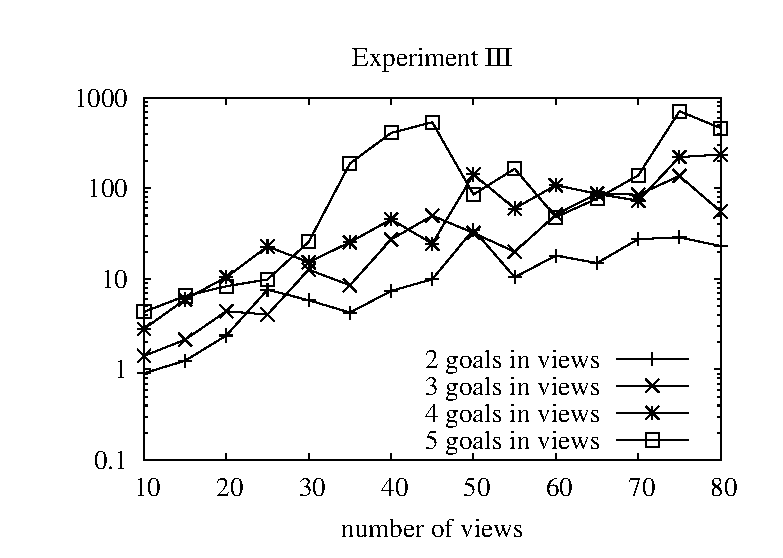
\includegraphics[width=.8\textwidth]{plots-v2/plot3}
\caption{Compilation times for random experiments with different number of views.
The plots are in logarithmic scale and the time is in seconds. }
\label{fig:random}
\end{figure}

\section{Related Work}

The problem of selecting the services that satisfy a user request is a
combinatorial optimization problem and several heuristics have been
proposed to find a good solution in a reasonably short period of
time~\cite{alrifaiR09,berardi08,myoung08,kuterG09,lecue09,rahmani08,sohrabiM09,Hiroshi2008}.

In a series of papers, Berardi and
others~\cite{berardi05,berardi08,berardi06} describe services and user
requests in terms of deterministic finite-state machines that are
encoded using Description Logics theories whose models correspond to
solutions of the problem, yet there are no efficient methods to compute
these models as in the case of SAT.

Ko et al.~\cite{myoung08} propose a constraint-based approach that encodes
the nonfunctional permissible
values as a set of constraints whose violation needs to
be minimized. Alrifai and Risse~\cite{alrifaiR09} develop a two-fold
solution that uses a hybrid integer programming algorithm to find the
decomposition of global QoS into local constraints, and then, selects
the services that best meet the local constraints.   

Recently, two planning-based approaches have been proposed. Kuter
and Golbeck~\cite{kuterG09} extend the SHOP2 planning algorithm to
select the trustworthy composition of services that implement a given
OWL-S process model, while Sohrabi and McIlraith~\cite{sohrabiM09}
propose a HTN planning-based solution where user preference metrics
and domain regulations are used to guide the planner into the space
of relevant compositions. Finally, L\'ecu\'e \cite{lecue09}  develops
a genetic-based algorithm to identify the composition of services
that best meet the quality criteria for a set of QoS parameters.

These existing solutions scale to a number of abstract concepts.
In addition to scalability, our approach provides a more expressive
framework where services are semantically
described in terms of domain ontology concepts, user preferences
restrict the space of solutions, and ontology relationships augment
the space of possible solutions. Finally, our approach is sound and
complete.

\Omit{
\subsection{Query Rewriting}

A number of algorithms have been developed to find the rewritings of a given query;
the most prominent being the Bucket algorithm \cite{levy:bucket}, the Inverse Rules
algorithm \cite{pods:DuschkaG97,Qian96}, the \minicon\ algorithm \cite{pottinger:minicon},
and the \mcdsat\ algorithm \cite{arvelo:aaai06}.
Generally, query rewriting algorithms work in two phases. During the first phase,
the algorithms identify the views that rewrite at least one sub-goal of the query, and
during the second, these partial rewritings are combined into complete rewritings.
The main difference between the algorithms is the criteria used to choose the relevant
views to reduce the space of non-useful rewritings.

The Bucket algorithm reduces the number of possibilities by just considering each
sub-goal in the query in isolation, and selecting the views that are able to produce
at least the attributes projected by the query. Since the attributes involved in the
joins in the query are not verified, a large number of rewritings comprised of Cartesian
products may be generated. 	

The Inverse Rules algorithm constructs a set of rules that invert the view definitions
and establish how to compute tuples for the database relations from the tuples of the
views. Similarly to the Bucket algorithm, it can produce a large number of non-useful
rewritings. 

The \minicon\ algorithm overcomes the limitations of the previous algorithms by identifying
only views that rewrite a set of the sub-goals of the query, and that can be combined with
the rest of the sub-goals. The key idea is to identify the mappings between the variables in
each sub-goal to the variables in one or more sub-goals in the views, in a way
that join variables in the query are mapped to join variables in the body of a view or to
the distinguished variables of the view. Mappings between variables and sub-goals are
represented in the so-called MiniCon Descriptions (MCDs) \cite{pottinger:minicon}.

Finally, the \mcdsat\ algorithm is able to identify the query rewritings of a query by
translating the problem of rewriting into the problem of enumerating the models of a
propositional theory whose models are in correspondence with the rewritings of the query.
The algorithm exploits the properties of d-DNNFs to efficiently enumerate the models of
the theory.
The \mcdsat\ algorithm has demonstrated to scale better than the \minicon\ algorithm over
a large number of benchmarks often showing performance improvements of several orders of
magnitude. However, the \mcdsat\ algorithm was not designed for rewriting problems
involving explicit constants, nor to compute the best rewritings with respect to a given
utility function or user preferences. We propose an extended encoding that 
overcomes these limitations and apply the encoding to SSP.

\subsection{Knowledge Compilation}

Knowledge compilation is the area in AI concerned with the problem of mapping
logical theories into suitable fragments that make certain desired operations
tractable \cite{cadoli:compilation}. Different compilation languages have been
defined, for instance, Ordered Binary Decision Diagrams (OBDDs) \cite{bryant:obdd},
Negation Normal Form (NNF) \cite{barwise:handbook}, and Decomposable Negation
Normal Form (DNNF) \cite{darwiche:map}. In this work, we make use of the properties
of the deterministic DNNFs (d-DNNF) \cite{darwiche:d-dnnfs} to provide an scalable
and efficient solution to the Service Selection Problem. 

A Negation Normal Form (NNF) theory is constructed from literals using only conjunctions
and disjunctions \cite{barwise:handbook}. An NNF is said to be decomposable (DNNF) \cite{darwiche:d-dnnfs} if for each conjunction, its variables are pairwise disjoint. A DNNF is said to be deterministic (d-DNNF) \cite{darwiche:d-dnnfs} if for each disjunction, the disjuncts are pairwise logically contradictory. A d-DNNF supports model counting in polytime in the size of its DAG, and model
enumeration in polytime in the size of the output.
Furthermore, given a literal ranking function $r$, one can compute the rank
of the best model in polytime for DNNFs \cite{darwiche:weighted}.

The fragments DNNF and d-DNNF are universal yet translating a CNF theory 
to DNNF format has an exponential cost in the worst case. This translation
is referred to as compilation in the field. There is a publicly available
compiler, called c2d,\footnote{\url{http://reasoning.cs.ucla.edu/c2d}}
that performs this compilation process and that makes
use of modern SAT techniques such as conflict-directed backtracking,
clause learning and caching \cite{darwiche:compiler}.
This compiler incurs in the worst case in exponential space in a parameter
called the width of the decomposition tree that is related to the ``connectivity''
of the CNF theory. However, in our experiments, the CNF theories that are
compiled are of low width.

\section{SSP Formalization into Logical Theories}
We use an approach similar to the one described in \cite{arvelo:aaai06} to
encode the SSP. We have limited space to make a comprehensive description of
the logical theory so the reader is referred there for details and formal results.

We identify service compositions  by enumerating the models of a logical
theory $\Delta=\Delta_{com}\cup\Delta_{id}^1\cup\cdots\Delta_{id}^N$
where $\Delta_{com}$ specifies how to combine $N$ independent copies theories
$\Delta_{id}$ that cover the goals in a user request $Q$.
Each $\Delta^i_{id}$ is a tagged copy $\Delta_{id}$ in which each literal
$\ell$ is tagged as $\ell^i$.
The Instantiation Description (ID) theory $\Delta_{id}$ consists of different
groups of clauses that guarantees that its models are in correspondence with
partial rewritings, while the theory $\Delta_{com}$ contains additional
clauses to guarantee a sound and complete combination of partial rewritings
into a complete rewriting.
The ID theory $\Delta_{id}$ consists of the following variables:
\begin{enumerate}[--]
\item $\{v_0,\ldots,v_n\}$ to indicate which source view $V_i$ is used, or $v_0$ to indicate the null ID.
\item $\{g_1,\ldots,g_m\}$ to indicate the goals covered by the view.
\item $\{z_{j,k,i}\}$ to indicate that the $j$th goal in $Q$ is covered by the $k$th goal in $V_i$.
\item $\{t_{x,y}\}$ to indicate that the variable/constant $x$ in $Q$ is mapped into the
      variable/constant $y$ in the view.
\end{enumerate}
The ranges of the indices for the $z$ and $t$ variables depend on the problem.

The following clauses encode the SSP problem in terms of the LAV mappings in $M$.
Rajaraman et al.\ \cite{RajaramanSU95} showed that for queries without negation or
arithmetic comparisons, but with constants, and $m$ goals and $k$ variables in the
head of the user request, it is enough to consider rewritings of length at most $N=m+k$.
\begin{enumerate}[C10.]
\item[C1.] (At least one view is used): $\bigvee_{i=0}^n v_i$.
\item[C2.] (At most one view is used): $\neg v_i\lor\neg v_j$ for $i\neq j$.
\item[C3.] (Null view equals null): $v_0 \Rightarrow \neg g_j$ for $1\leq j\leq m$.
\item[C4.] (Views are useful): $v_i \Rightarrow \bigvee_{j=1}^m g_j$ for $1\leq i\leq n$.
\item[C5.] (Subgoals covered at most once): $z_{j,k,i} \Rightarrow \neg z_{j,l,i}$ for appropriate $i,j,k,l$.
\item[C6.] (Scope of views): $v_i \Rightarrow \neg g_j$ for goals that cannot be covered by $V_i$.
\item[C7.] (Consistency): $v_i \land g_j \Leftrightarrow \bigvee z_{j,k,i}$ for appropriate $i,j,k$.
\item[C8.] (Dead variables): $v_i \Rightarrow \neg t_{x,y}$ for all $x,y$ with $y\notin V_i$.
\item[C9.] (1-1 for $\exists$ vars): $v_i \land t_{x,y} \Rightarrow \neg t_{x,y'}$ for all
           existential variables $y,y'\in V_i$.
\item[C10.] (Distinguished): $v_i \Rightarrow \neg t_{x,y}$ for distinguished $x$ and existential
            $y\in V_i$.
\item[C11.] (Existential): $v_i\land t_{x,y}\Rightarrow g_j$ for exist.\ $y\in V_i$ and
            goals $g_j$ that contain $x$.
\item[C12.] (Match): $v_i\land z_{j,k,i} \Rightarrow t_{x,y}$ for all $x,y$ that must match
            if $g_j$ is covered by goal $k$ in $V_i$.
\item[C13.] (If all vars in $V_i$ are distinguished, it covers only one goal):
            $v_i \land g_j \Rightarrow \neg g_k$ for appropriate views $v_i$.
\end{enumerate}
These clauses are the same clauses used by \mcdsat\ to encode QRPs \cite{arvelo:aaai06}.
In order to properly manage constant symbols, the clauses must be enhanced with:
\begin{enumerate}[C10.]
\item[C14.] (Direct inconsistency 1): $t_{x,A} \Rightarrow \neg t_{x,B}$.
\item[C15.] (Direct inconsistency 2): $t_{A,x} \Rightarrow \neg t_{B,x}$.
\item[C16.] (Direct inconsistency 3): $\neg t_{A,B}$.
\item[C17.] (Transitivity 1): $v_i\land t_{A,y}\land t_{x,y}\land t_{x,z}\Rightarrow t_{A,z}$.
\item[C18.] (Transitivity 2): $v_i\land t_{y,A}\land t_{y,x}\land t_{z,x}\Rightarrow t_{z,A}$.
\end{enumerate}
Recall that, as shown in Section~2, the main issue when handling
constants is to be sure that not two different constants are mapped
into each other either directly or indirectly.
Clauses C14--C16 prune direct inconsistent mappings, while the last
two clauses implement a restricted propagation of mappings that prune
indirect inconsistencies.
Likewise, the theory $\Delta_{com}$ that specifies complete
instantiations contains the following clauses:
\begin{enumerate}[C10.]
\item[C19.] (Cover all goals): $\bigvee_{j=1}^m g^i_j$ for $1\leq i\leq N$.
\item[C20.] (Disjunctive cover): $g^i_k \Rightarrow \neg g^j_k$ for $i\neq j$.
\item[C21.] (Prune symmetries): $g^i_j \Rightarrow \bigvee_{k=1}^{j-1} g^{i-1}_k$
            for $1\leq j\leq m$ and $1\leq i\leq N$.
\item[C22.] (Direct inconsistency 4): $t^i_{x,A} \Rightarrow \neg t^j_{x,B}$.
\end{enumerate}
These clauses provide a sound and complete characterization of SSPs in the
sense that their models are in correspondence with the rewritings of the user request.

For the QoS parameters, we assume a simple additive aggregation model in
which each view $V_i$ is associated with a cost $c(V_i)$ (negative if utility),
and a complete rewriting with the sum of the cost of its views. User preferences rules are transformed into propositional logic formulas whose cost is a high number.
An optimal or best solution is one with minimum cost, and the
optimal value of the SSP is the cost of an optimal rewriting.
A SSP always has a well-defined optimal value (if there are no rewritings,
its cost is $\infty$), but it may have multiple best rewritings.
The SSP with costs consists in finding all optimal rewritings or
one rewriting, this depends on the particular application.
In our formulation, this can be done from the d-DNNF that encodes $\Delta$
using the literal ranking function $r$ that assigns $r(\ell)=c(V_i)$ if
$\ell=v_i$, and $r(\ell)=0$ if $\ell\notin\{v_1,\ldots,v_n\}$.
}

\section{Discussion}

We proposed a novel formalism for expressing Service Selection Problems
involving an ontology of generic concepts, services described using views
in terms on the concepts, following the LAV approach, and user's preferences.
This is a general, well-defined and scalable framework since it is based
on logic, the LAV approach, and permits the modeling of real-life scenarios
and preferences.

We also showed how the propositional theory used in \mcdsat\ for solving
the QRP can be extended to handle SSPs.
This formulation allows to exploit the properties of modern SAT solvers
to provide an efficient and scalable solution to the SSP.

The preliminary experiments show that the approach can be applied to
real-sized problems. We are currently working on a complete implementation
of the formalism in order to offer its full expressiveness.
In the future, we plan to use other off-the-shelf SAT tools such 
as MiniMaxSat that is able to find a best model without the need 
to compile the CNF into d-DNNF.

\bibliographystyle{abbrv}
\bibliography{ref}

\end{document}

